\chapter{OAuth}

Nelle applicazioni odierne si utilizzano spesso le \textit{API}, che permettono
all'applicazione di ottenere accesso a dati e servizi di valore. Per questo motivo
è necessario restringere l'accessi delle API a gruppi autorizzati. Serviranno dunque
delle autorizzazioni per chiamare le API. Nel passato un utente spesso doveva condividere
le proprie credenziali con l'applicazione per assicurarsi che tale chiamata API
funzionasse correttamente. Questo forniva alle applicazioni una quantità di dati
eccessiva e costringeva i creatori dell'applicazione di avere la responsabilità
della salvaguardia dei dati sensibili. Osserveremo ora come il framework
\textbf{OAuth 2.0} fornisca una soluzione migliore per autorizzare le applicazioni
ad effettuare chiamate alle API.

\section{API Authorization}

Un applicazione potrebbe aver bisogno di chiamare un API per conto di un utente
per accedere a contenuti posseduti dall'utente o per conto proprio se l'applicazione
possiede i contenuti desiderati.

\begin{figure}[H]
      \centering
      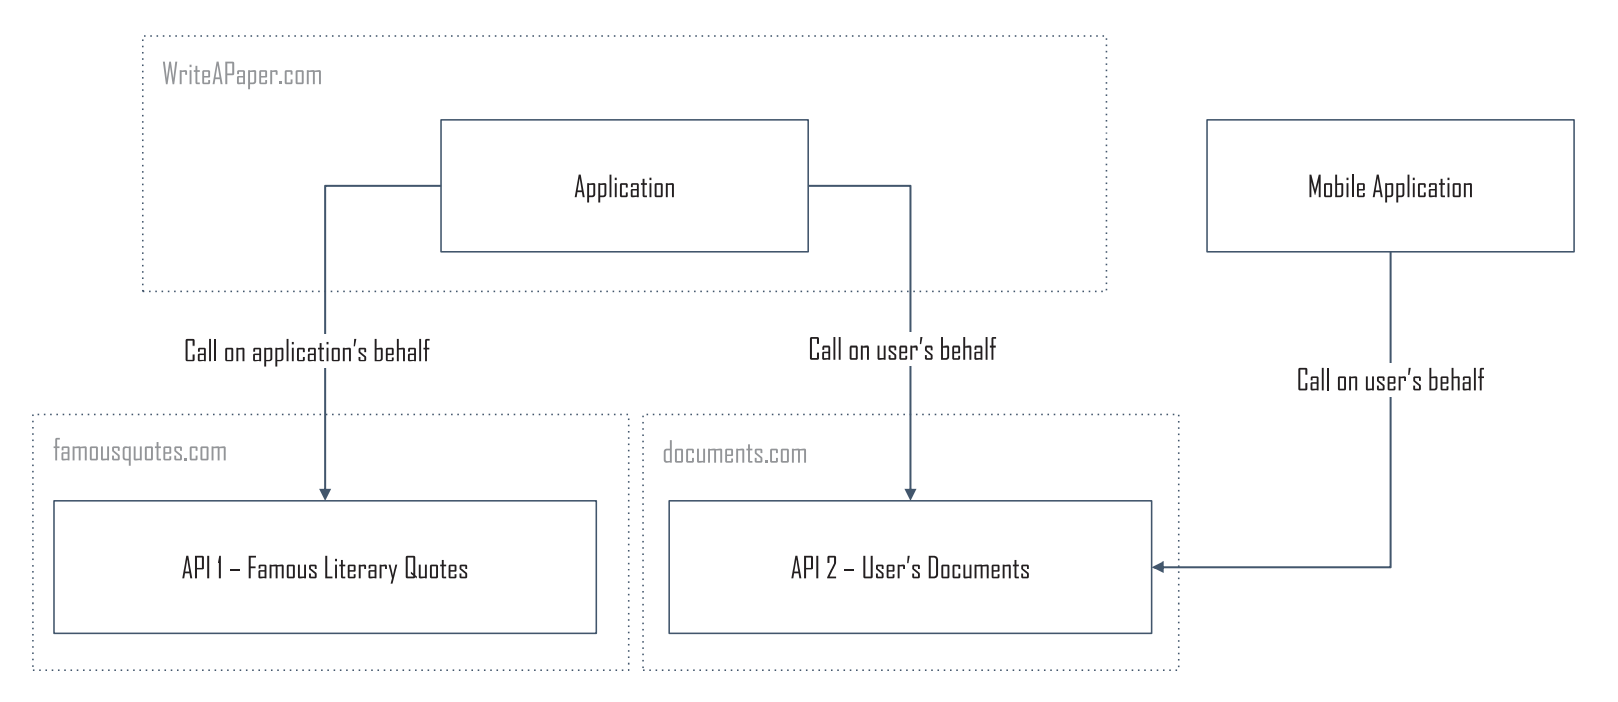
\includegraphics[width=\textwidth, keepaspectratio]{capitoli/id_managing/imgs/api1.png}
      \caption{API Authorization: user-based vs client-based flow.}
\end{figure}

\section{Cos'è ?}

OAuth 2.0 fornisce una soluzione di autorizzazione, ma non di autenticazione. Consente
all'applicazione di chiamare un API per conto proprio o dell'utente e tale chiamata
avrà lo scope che è vincolato alla richiesta di autorizzazione. Lo step di
autenticazione in OAuth 2.0 controlla se l'utente ha privilegi necessari per
autorizzare una richiesta di accesso ad una risorsa particolare dopodiché, se
questo accesso è consentito, il server genererà un token di autorizzazione che
verrà utilizzato da OAuth 2.0 per recuperare i dati richiesti.\\
Lo scopo del token di accesso di OAuth 2.0 è solo quello di permettere l'accesso alle
API e non fornisce alcuna informazione riguardo l'evento di autenticazione o riguardo
all'utente.
Si vede dunque che l'utilizzo di OAuth 2.0 è appropriato solamente per autorizzare
solamente chiamate di API. È tuttavia possibile effettuare modifiche proprietarie al
protocollo di base per implementare un opzione di autenticazione. Un esempio è
OIDC.

\begin{figure}[H]
      \centering
      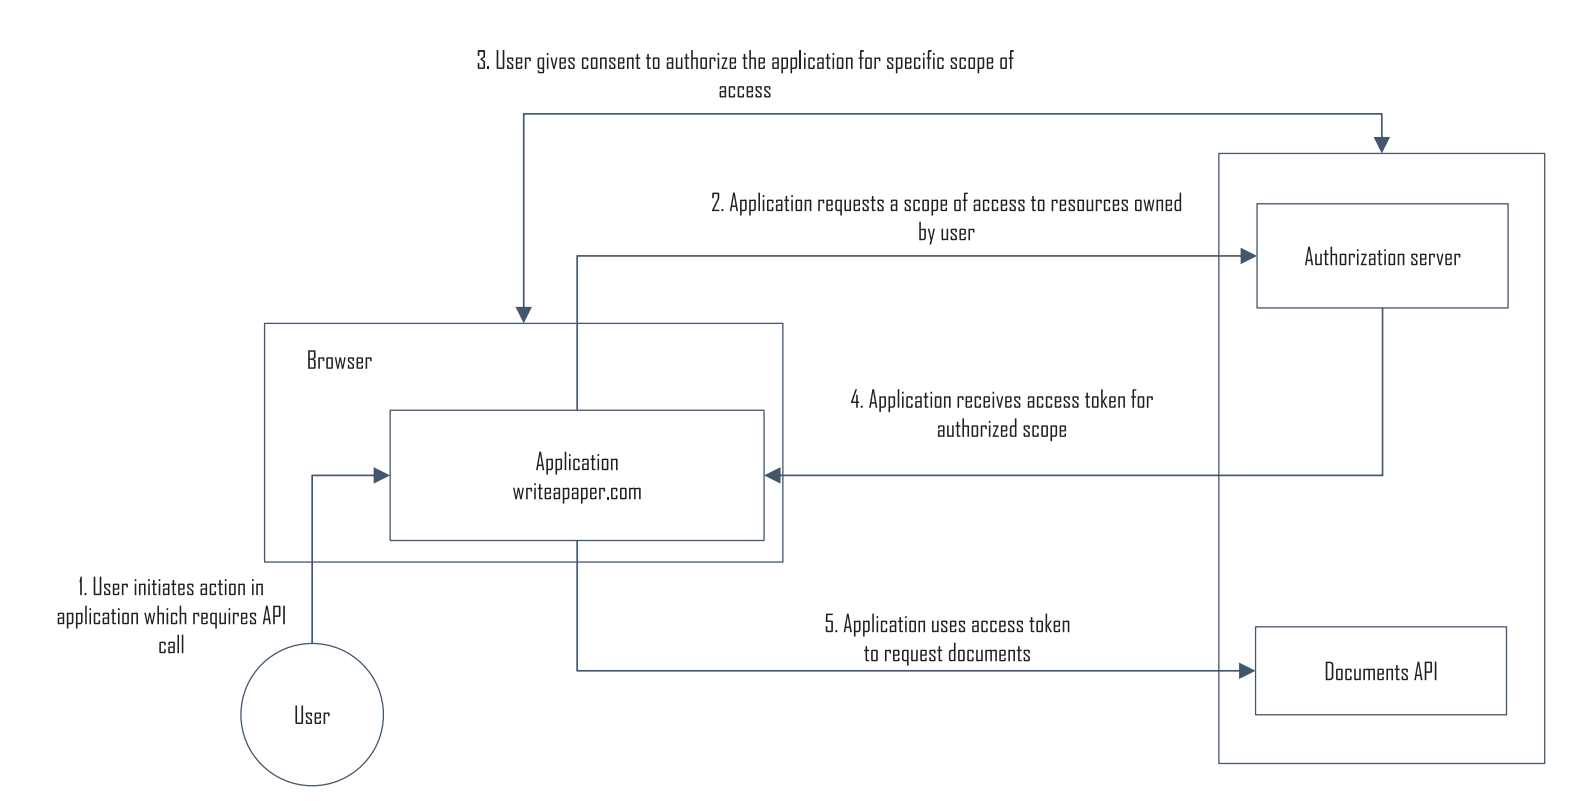
\includegraphics[width=\textwidth, keepaspectratio]{capitoli/id_managing/imgs/api2.png}
      \caption{Flow di esecuzione con OAuth 2.0.}
\end{figure}

\section{Terminologia}

Introduciamo ora alcune definizioni e terminologia per analizzare più in dettaglio
OAuth 2.0.

\subsection{Roles}

OAuth 2.0 definisce 4 ruoli per la richiesta di autorizzazione:

\begin{itemize}
      \item \textbf{Resource Server}: un servizio che salva le risorse protette affinché
            possano essere richieste da un'applicazione.
      \item \textbf{Resource Owner}: un utente o altre entità che possiede risorse protette
            nel resource server.
      \item \textbf{Client}: un'applicazione che vuole l'accesso a delle risorse nel
            resource server. Sinonimo di \textit{Applicazione}.
      \item \textbf{Authorization Server}: un servizio di cui il resource server si fida
            affinché possa autorizzare le applicazioni a chiamare il resource server.
            Autentica l'applicazione o il resource owner e richiede il consenso dell'utente
            se l'applicazione
            vuole fare una richiesta per suo conto. Con OAuth 2.0 i resource server fa
            affidamento all'authorization server e a volte possono operare come una
            singola entità.
\end{itemize}

\subsection{Tipi di Client}

In OAuth 2.0 ci sono 2 tipi di client:

\begin{itemize}
      \item \textbf{Confidential Client}: un'applicazione che viene eseguita su un server
            protetto può salvare in maniera sicura informazioni confidenziali per
            autenticare se stessa con un authentication server.
      \item \textbf{Public Client}: un'applicazione che viene eseguita primariamente sul
            dispositivo dell'utente e non può salvare in maniera sicura dati confidenziali
            e può autenticarsi con il server solo tramite OAuth.
\end{itemize}

\subsection{Client Profiles}

In OAuth 2.0 ci sono 3 tipi di profili in base alla tipologia di applicazione:

\begin{itemize}
      \item \textbf{Web Application}: un client confidenziale con il codice che viene
            eseguito su un server di backend protetto. Il server può salvare in maniera
            sicura qualunque segreto necessario al client per autenticarsi e anche i
            token ottenuti dall'authorization server.
      \item \textbf{User Agent-Based App}: si presume sia un client pubblico con codice
            che viene eseguito nel browser dell'utente. Un esempio è una pagina web
            basata su Javascript.
      \item \textbf{Native Application}: si presume sia un client pubblico installato
            ed eseguito sul dispositivo dell'utente come un'applicazione mobile.
\end{itemize}

\subsection{Token e Codici di Autorizzazione}

In OAuth 2.0 ci sono 2 token di sicurezza e un token di autorizzazione intermedio:

\begin{itemize}
      \item \textbf{Authorization Token}: un codice opaco intermediario ritornato
            da un'applicazione ed utilizzato per ottenere un token di accesso e
            opzionalmente un token di refresh. Ogni authorization code è utilizzato
            una volta.
      \item \textbf{Access Token}: un token utilizzato da un'applicazione per accedere
            a un API. Rappresenta l'autorizzazione dell'applicazione per chiamare un API
            ed ha una scadenza.
      \item \textbf{Refresh Token}: un token opzionale che può essere utilizzato da
            un'applicazione per richiedere un nuovo access token quando uno precedente
            è scaduto.
\end{itemize}

\section{Come funziona ?}

A seconda del caso d'uso, OAuth 2.0 dispone di 4 metodologie con cui può richiedere
l'autorizzazione per chiamare un API. Le credenziali da recuperare sono conosciute
anche con il nome \textit{permessi di autorizzazione} (\textbf{authorization grants}).

\begin{itemize}
      \item \textbf{Authorization Code Grant}
      \item \textbf{Implicit Grant}
      \item \textbf{Resource Owner Password Credential Grant}
      \item \textbf{Client Credential Grant}
\end{itemize}

Analizziamoli in maggiore dettaglio.

\subsection{Authorization Code Grant}

Questo tipo di autorizzazione utilizza due richieste dall'applicazione all'authorization
server per ottenere l'access token.\\
Nella prima richiesta il browser dell'utente viene reindirizzato all'end point di
dell'authorization server con la richiesta di autorizzare un api call da parte
dell'utente.
Questo reindirizzamento consente all'authorization server di interagire con l'utente
per farlo autenticare. Dopo aver ottenuto il consenso, l'utente viene reindirizzato
all'applicazione
con l'authorization conde. L'applicazione utilizzerà questo codice per mandare una
backchannel request all'authorization server per ottenere l'access token.
L'authorization server risponderà con un access token che verrà utilizzato per
chiamare le API

\begin{figure}[H]
      \centering
      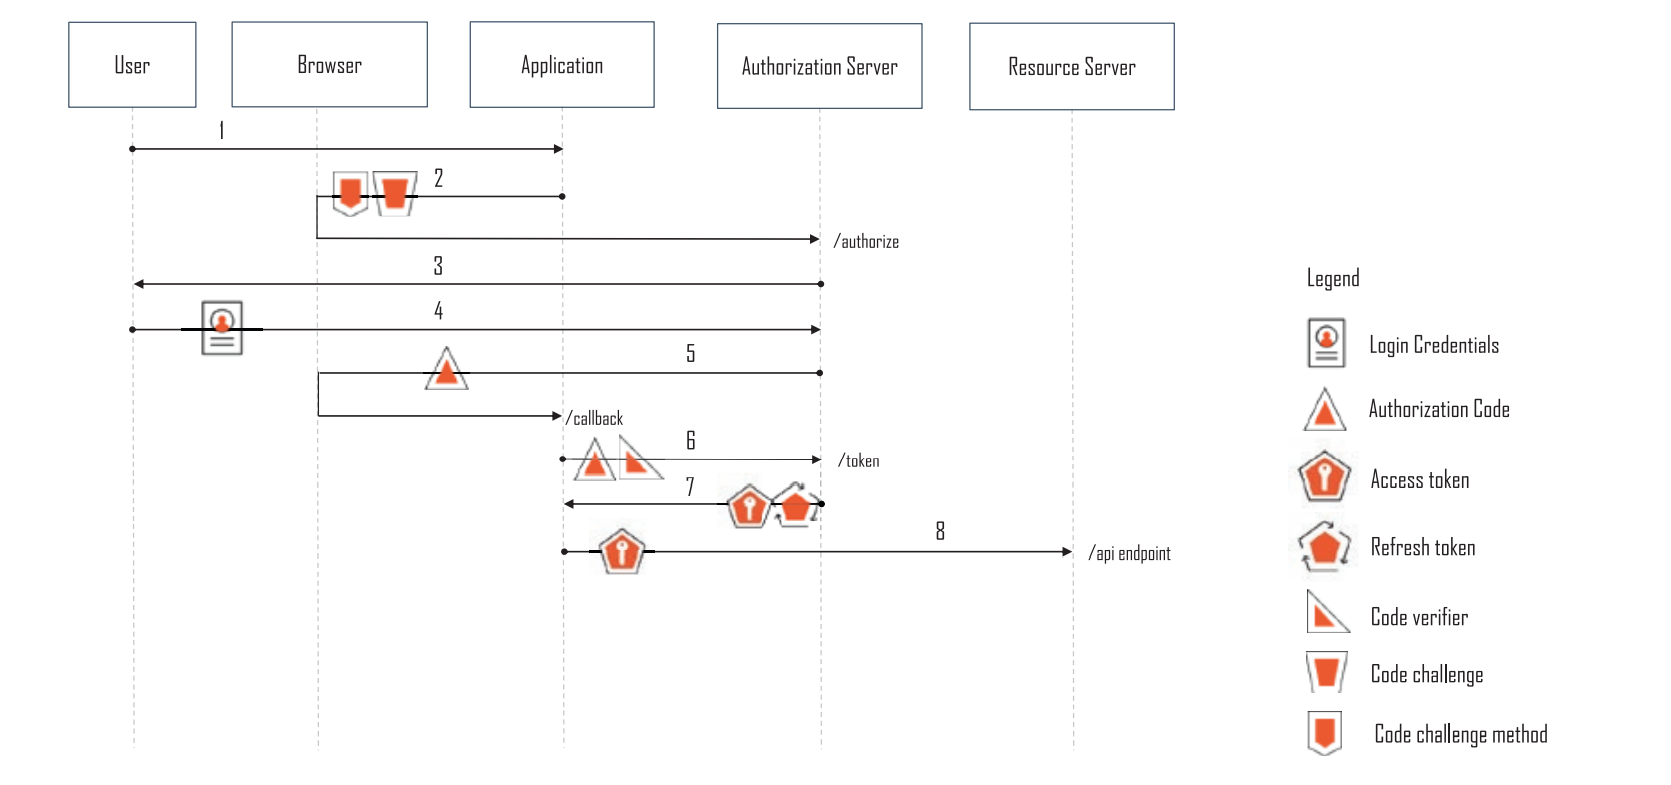
\includegraphics[width=\textwidth, keepaspectratio]{capitoli/id_managing/imgs/pkce.png}
\end{figure}

\begin{enumerate}
      \item L'utente accede all'applicazione,
      \item L'applicazione reindirizza il browser all'endpoint di autorizzazione
            dell'authorization server con una richiesta di autorizzazione,
      \item L'authorization server richiede all'utente l'autorizzazione e il consenso,
      \item L'utente si autentica e fornisce il consenso per la richiesta,
      \item L'authorization server reindirizza il browser dell'utente all'applicazione
            con l'authorization code,
      \item L'applicazione chiama l'authorization server token endpoint passandogli
            il codice di autorizzazione,
      \item L'authorization server risponde con un access token,
      \item L'applicazione chiama il resource server (API) utilizzando l'access token.
\end{enumerate}

Questo tipo di autorizzazione era originariamente ottimizzata per i
client confidenziali, però con l'aggiunta di \textbf{PKCE} può essere utilizzata anche dai
client pubblici.

\subsubsection{Authorization Code Grant + PKCE}

Il meccanismo \textit{Proof of Key for Code Exchange} (PKCE) permette di assicurarsi
che l'applicazione che ha richiesto il codice di autorizzazione è la stessa che lo
utilizza per ottenere l'access token. Questo vuol dire che PKCE serve per proteggersi
da potenziali intercettazioni delle richiesti di autorizzazione.
Per poter utilizzare PKCE l'applicazione crea una stringa crittografata in maniera
aleatoria chiamata \textbf{code verifier}. L'applicazione poi calcola un valore derivato
chiamato \textbf{code challenge} dal code verifier. Quando l'applicazione manda un
authorization request in due step manda questo code challenge insieme al metodo utilizzato
per derivarlo e quando manda l'authorization code per ottenere l'access token manda anche
il code verifier. L'authorization server confronta i valori ricevuti e vede se
il code verifier può essere utilizzato per ottenere il code challenge mandato in precedenza,
se si vorrà dire che sono mandati dalla stessa macchina.\\

Ci sono due metodi per ottenere il code challenge:

\begin{itemize}
      \item \textbf{plain}: il code challenge è uguale al code verifier, dunque non c'è
            protezione per la compromissione del code challenge.
      \item \textbf{s256}: è quello che andrebbe utilizzato, è un metodo che utilizza
            una codifica dell'url in base 64 con SHA256 per proteggere il code verifier.
\end{itemize}

\subsection{Implicit Grant}

Questo tipo di grant era utilizzato quando lo standard CORS (Cross-Origin Resource
Sharing) non era ancora ampiamente utilizzato, quindi le pagine web potevano solo
fare richieste al dominio in cui erano caricate. Questo implicava che non era possibile
chiamare il token endpoint dell'authorization server, dunque l'authorization server
risponde all'authorization request fornendo direttamente l'authorization token come
frammento di un redirect url codificato in hash.
Questo tipo di grant è ottimizzato per l'utilizzo con public client.

\begin{figure}[H]
      \centering
      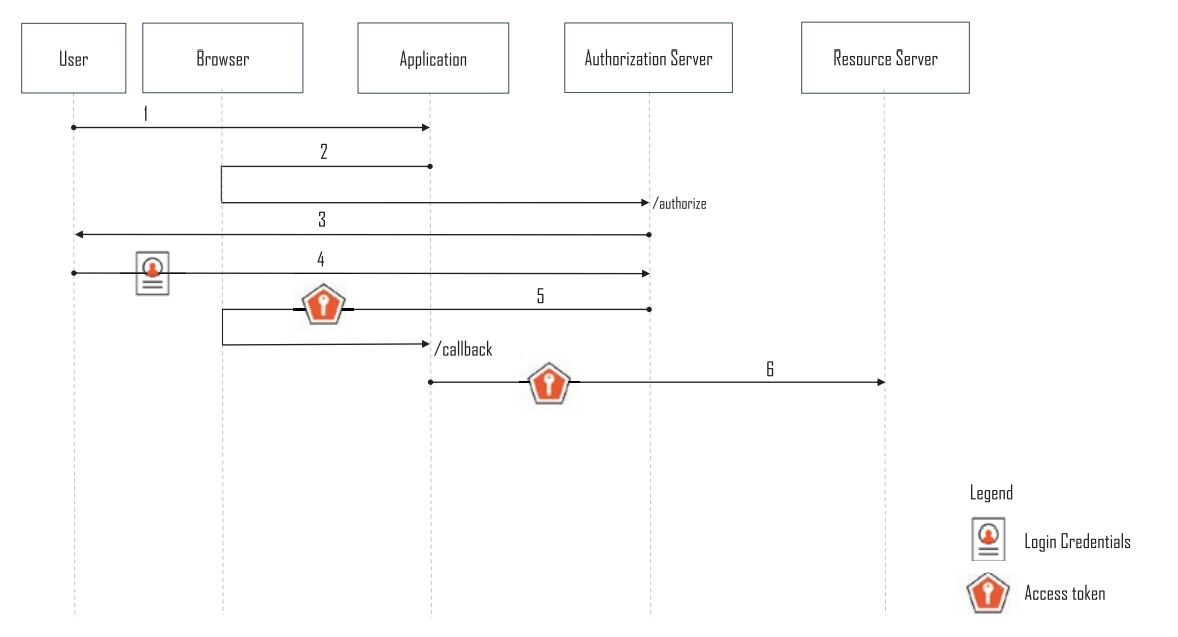
\includegraphics[width=\textwidth, keepaspectratio]{capitoli/id_managing/imgs/implicitgrant.png}
\end{figure}

\begin{enumerate}
      \item L'utente accede all'applicazione.
      \item L'applicazione reindirizza il browser all'authorize endpoint
            dell'authorization server con la richiesta di autorizzazione.
      \item L'authorization server richiede all'utente di autenticarsi e fornire consenso.
      \item L'utente si autentica e fornisce il consenso.
      \item L'authorization server reindirizza al callback dell'applicazione fornendo
            l'access token.
      \item L'applicazione utilizza l'access token per chiamare le API.
\end{enumerate}

\subsection{Resource Owner Password Credential Grant}

Il resource owner password credential grant è un tipo di grant che non richiede che
l'utenti si interfacci con l'authorization server poiché le credenziali dell'utente
finale vengono gestite direttamente dall'applicazione. L'utilizzo di questo
tipo di grant è sconsigliato poiché espone le credenziali dell'utente a potenziali rischi.
Inoltre, non è previsto uno step in cui l'utente fornisce il consenso ad utilizzare parte
dei dati, dunque l'applicazione può richiedere qualsiasi dato voglia e l'utente non ha
modo di prevenire un abuso delle proprie credenziali.

\begin{figure}[H]
      \centering
      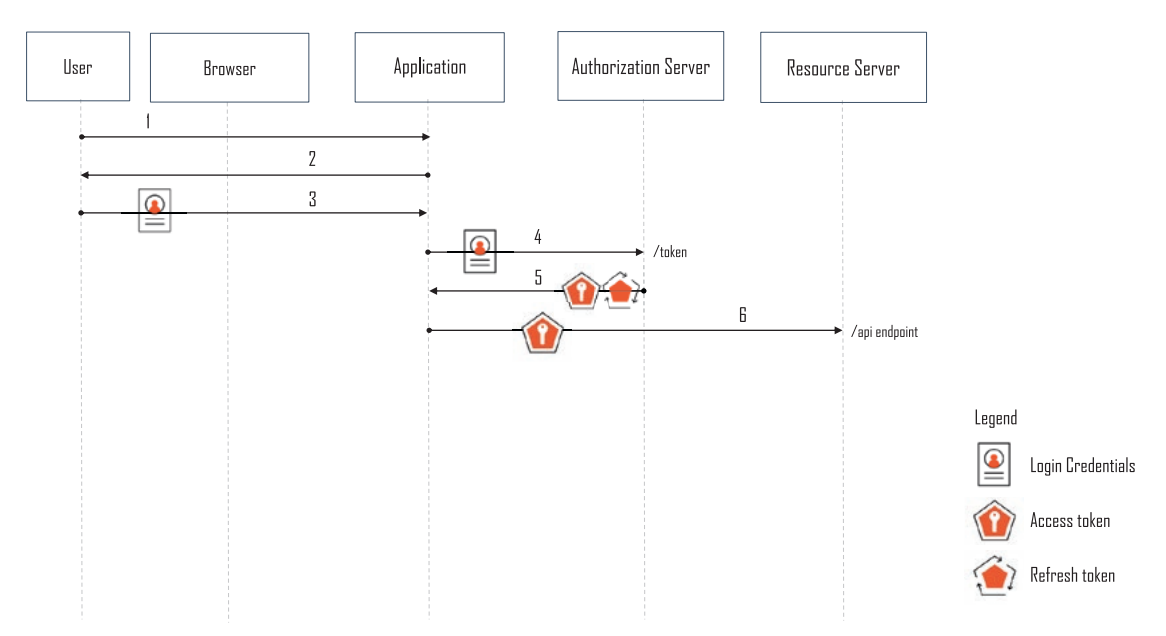
\includegraphics[width=\textwidth, keepaspectratio]{capitoli/id_managing/imgs/passgrant.png}
\end{figure}

\begin{enumerate}
      \item L'utente accede all'applicazione.
      \item L'applicazione richiede all'utente le credenziali.
      \item L'utente fornisce le credenziali all'applicazione.
      \item L'applicazione manda una token request al token endpoint dell'authorization
            server con le credenziali dell'utente.
      \item L'authorization server risponde con un access token.
      \item L'applicazione chiama l'API utilizzando l'access token
\end{enumerate}

L'unico scenario in cui questi tipo di grant è minimamente sensato è quello della
migrazione di un identità da una piattaforma all'altra che hanno codifiche hash
incompatibili, anche in questo caso ci sono comunque metodi migliori.

\subsection{Client Credential Grant}

Questo tipo di grant è utilizzato quando un'applicazione fa una richiesta API per
ottenere risorse che sono possedute dall'applicazione.

\begin{figure}[H]
      \centering
      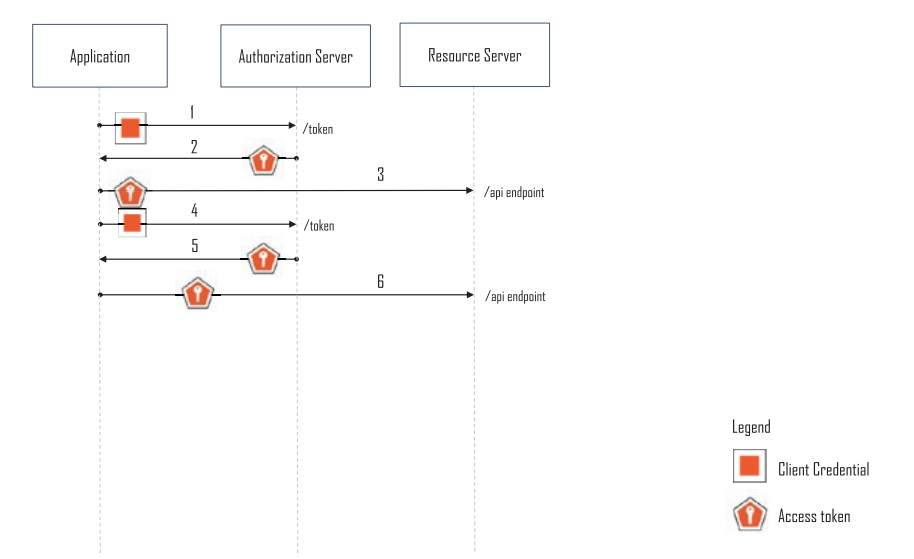
\includegraphics[width=\textwidth, keepaspectratio]{capitoli/id_managing/imgs/clientgrant.png}
\end{figure}

\begin{enumerate}
      \item L'applicazione manda una richiesta di autorizzazione includendo le credenziali
            dell'applicazione all'authorization server.
      \item L'authorization server valida le credenziali e risponde con un access token.
      \item L'applicazione chiama le API utilizzando l'access token.
      \item Gli step precedenti si ripetono se l'access token è scaduto quando vengono chiamate
            le API.
\end{enumerate}

\section{Chiamare le API}

Una volta ottenuto il token l'applicazione può effettuare le chiamate API e tipicamente
è fatto utilizzando la richiesta HTTP "Authorization" e specificando l'access token
nel campo \verb|Authorization| dell'header.

\begin{lstlisting}
   GET /api-endpoint HTTP/1.1
      Host: api-server.com
      Authorization: Bearer <access_token>
\end{lstlisting}

L'access token ha un tempo di scadenza per ottimizzare le performance, a volte
può essere anche salvato in cache fin quando non scade. È importante fornire
all'access token  l'appropriato scope di privilegi per le chiamate API.

\section{Refresh Token}

L'access token ha una scadenza e può essere utilizzato solo per un tempo limitato,
ma non ha un limite sul numero di volte che può essere utilizzato.
Questo permette di migliorare le performance se il token viene salvato in cache.
Per migliorare ulteriormente le performance durante l'autorizzazione può essere
richiesto un token aggiuntivo, il \textbf{refresh token}, il cui scopo è quello di
riottenere un access token una volta scaduto. Potrebbe sembrare intelligente
refreshare l'access token appena scade, ma in pratica risulta essere più sicuro
effettuare il refresh solo quando il token è necessario.
In alcuni server il refresh avviene in automatico, in altri invece ci si aspetta
che la richiesta avvenga in maniera esplicita da parte dell'applicazione.